\chapter{Feature selection}\label{ch:fs}

We introduce in this chapter the concepts of feature selection and false discovery rate control,
as well as a short review of a few methods that are usually employed,
including the Lasso and Benjamini–Hochberg-Yekutieli procedures.

\section{Background on feature selection}\label{sec:bfs}

\subsection{Definitions}\label{subsec:fs_defs}

Feature selection primarily consists in identifying the most relevant features (or covariates)
explaining an observed variable.
It is closely related to Occam's razor which is a principle stating that
the simplest explanation is often the best one.
More formally, let $\cX$ be a $p$-dimensional random vector representing observed features
and $\cY$ a random target that may depend on $\cX$.
For example, $\cX$ could be the expression levels of the genes of an individual,
and $\cY \in \zoset$ a binary response indicating whether or not the person has some disease.
We wish to find the subset of covariates $\cS \subseteq \fset$ that best explains the target $\cY$,
be it a numerical or a categorical variable.
The notion of relevance of a feature $\cX_j$ can be captured by the dependence of $\cY$ on $\cX_j$.
To do so, suppose that the joint vector $\left( \cX,\, \cY \right)$ follows some distribution,
that is $\left( \cX,\, \cY \right) \sim \mathcal{P}_{\cX,\, \cY}$.
Even though finding the full conditional distribution $\cP_{\cY \mid \cX}$ is beyond hope in general,
one may be interested in finding on which subset $\cS$ of features $\cP_{\cY \mid \cX}$ depends.
As this set is not necessarily unique,
the principle of parsimony motivates us to find the smallest one.
In other words, we are interested in finding the smallest subset $\cS$ such that
$\cY \mid \left\{ \cX_j \right\}_{j \in \cS}$ is independent of $\left\{ \cX_j \right\}_{j \notin \cS}$.
Such a subset is called a Markov Blanket~\citep{markov_blanket, markov_blanket_fs}
and is not necessarily unique and may not even exist.
\begin{figure}[h]
    \centering
    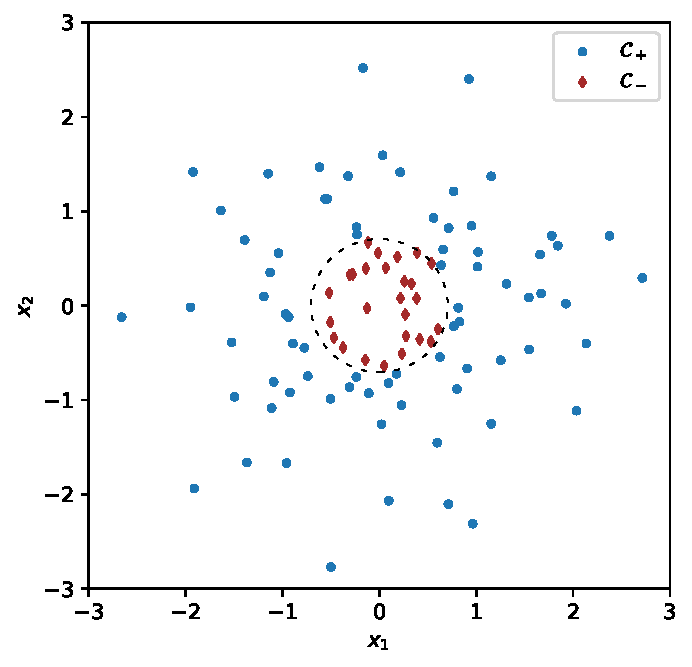
\includegraphics[width=0.4\linewidth]{figures/fs_subset_not_unique.pdf}
    \caption{
        Illustration of the non-uniqueness of the Markov blanket.
        Here $\cX_1 \sim \cN\left( 0,\, 1 \right)$
        and $\cX_2 \sim \cN\left( 0,\, 1 \right)$ are independent,
        $\cZ = \cX_1^2 + \cX_2^2$.
        $\cY$ is $\cC_+$ if $\cZ \geq \frac{1}{2}$,
        $\cC_-$ otherwise.
        The target $\cY$ can be predicted directly from both the pair $\left( \cX_1,\, \cX_2 \right)$
        or the distance to origin $\cZ$ alone.
    }
    \label{fig:fs_subset_not_unique}
\end{figure}
We define the set of null features $\cH_0 \subseteq \fset$ as follows:
$j \in \cH_0$ if and only if $\cY \independent \cX_j \mid \cX_{-j}$
(where $\cX_{-j}$ denotes that all vector entries are kept except the $j$th).
The goal is thus to find a procedure selection a subset of features
$\hat{\cS} \subseteq \fset$.

As a matter of example,
in the case of linear regression where we assume that the target and the features follow a linear relationship
\begin{equation*}
    \cY = \cX^\top \bbeta + \epsilon
\end{equation*}
where $\bbeta \in \R^p$ and $\epsilon$ is a gaussian noise,
feature selection would consist in identifying which coefficients of $\bbeta$ are non null.

In practice, one would observe several independent realizations of
$\left( \cX,\, \cY \right)$ and would aggregate them into a feature matrix
$X \in \R^{n \times p}$ of $n$ samples and $p$ features, and a target vector $\yy \in \R^n$ respectively.
The independence of the observations is a credible assumption in many real life settings

\subsection{Motivation}\label{subsec:fs_motivation}

Feature selection may be used in a multitude of contexts and we point out here the main benefits of
performing it on a dataset.
\begin{enumerate}
    \item \textit{Making a model more interpretable.}
    It gives insights on the most relevant features to explain the observed target.
    It is for instance decisive when you are interested in the role of genes.
    \item \textit{Facilitating data visualization.}
    When only a small subset of the features is selected,
    projecting it to a low (2 or 3) dimensional space is easier.
    \item \textit{Reducing the training time.}
    Many machine learning algorithm have a super-linear time complexity in the number of features.
    Pre-selecting a small subset with a cheaper method can noticeably as less\citep{high_dimensional_fs}.
    \item \textit{Improving the generalization of machine learning models.}
    Irrelevant features may only be noise and fitting a model against them at train time
    is prone to over-fitting noise.
    \item \textit{Avoiding the curse of dimensionality}~\citep{curse_dimensionality}.
    For example, the $k$-nearest neighbors algorithms~\citep{knn} is known to perform badly as the feature space
    dimension increases.
    The number of samples actually has to grow exponentially in the number of features in order for the algorithm
    to perform decently.
\end{enumerate}
Recently, the cost of measuring more features has drastically decreased.
Many datasets, and especially in biology, end up with several dozens of thousands of features.
Most of these features are expected to be insignificant, but there is a priori no reason to eliminate them.
Adding them to the feature matrix is cheap, and it is then the role of the machine learning algorithm
to detect the relevant ones.

\subsection{Techniques}\label{subsec:fst}

A lot of different paradigms and techniques to perform feature selection exist~\cite{intro_fs}
a~\cite{fs_text_classification}.
b\cite{gene_selection_cancer_svm}
c\cite{fs_for_classification}
d\cite{fs_for_classification_a_review}

\subsubsection{Lasso}\label{subsubsec:lasso}

First rediscovered by~\cite{lasso},
the Lasso has become increasingly popular because of its capacity to both shrink
the coefficients towards 0 and to select a subset of the features.
It is basically a linear least squares regression whose weights are penalized by their $\ell_1$ norm,
multiplied by some factor $\lambda > 0$.
%
\begin{equation}\label{eq:lasso}
    \hat{\bbeta}(\lambda) =
    \underset{\bb}{\argmin}\;
    \frac{1}{2}\norm{\yy - X\bb}_2^2 + \lambda\norm{\bb}_1
\end{equation}
%
The $\ell_1$ penalty tends to make the weights $\hat{\bbeta}(\lambda)$ sparse as $\lambda$ increases.
Actually, for any feature $j$,
there is a $\lambda_{\min}$ such that for all $\lambda \geq \lambda_{\min}$,
$\hat{\bbeta}_j(\lambda) = 0$.
That wouldn't be the case with an $\ell_2$ penalty,
for which the coefficients tend to $0$ without reaching that value.
This property makes the Lasso particularly suited for feature selection;
just keep the features whose weight is non-zero.
However, the choice of $\lambda$ seems to be arbitrary,
especially as it's not possible to know beforehand how many features will be selected.

The behavior of the path $\lambda \mapsto \hat{\bbeta}(\lambda)$ has been extensively studied,
and the algorithm LARS~\cite{lars} was developed to efficiently compute it,
which is possible because it is piecewise linear.
It allows to compute $\hat{\bbeta}$ for all relevant value of $\lambda$ at a marginal cost.
In practice, the $\lambda$ giving the highest score on a \emph{train} dataset is picked.
The $\ell_1$ regularization can easily be extended to many other estimators than the least squares,
as for example logistic regression or SVMs.

\subsubsection{Sparse center classifiers}

Nearest centroid classification~\citep{centroid_classification} is a very simple classification scheme.
It consists in computing the averages $\btheta^\pm = \sum_{j \in \cI^\pm} \xx_i \in \R^p$
of the data points from the positive and negative classes $\cC^\pm$,
where $\cI^\pm$ contain the positive and the negative points.
A new data point $\xx \in \R^p$ is classified positive or negative depending on its closest average
$\btheta^+$ or $\btheta^-$.
Finding the class averages can be formulated as the following optimization problem.
\begin{equation}\label{eq:centroids_averages}
    \argmin_{\btheta^+, \btheta^-}
        \frac{1}{n^+} \sum_{i \in \cI^+} \big\lVert \xx_i - \btheta^+ \big\rVert^2_2
        + \frac{1}{n^-} \sum_{i \in \cI^-} \big\lVert \xx_i - \btheta^- \big\rVert^2_2
\end{equation}
Note $\Delta$ the decision boundary,
such that $\xx$ is classified $\cC^+$ if $\Delta\left( \xx \right) > 0$ and $\cC^-$ otherwise.
\begin{equation}\label{eq:centroids_boundary}
    \Delta(\xx) = \norm{\xx - \btheta^-}^2_2 - \norm{\xx - \btheta^+}^2_2
\end{equation}
The expression~\ref{eq:centroids_boundary} can be expanded into
$\Delta(\xx) = \norm{\btheta^+}^2_2 + \norm{\btheta^-}^2_2 + 2\xx^\top(\btheta^+ - \btheta^-)$,
making it clear that the decision depends on the feature $j$ if and only if $\btheta^+_j \neq \btheta^-_j$.
Using this observation,\cite{sparse_center_classifiers} introduced a $\ell_0$ penalized version
of~\ref{eq:centroids_averages} that can be solved very efficiently in closed-form.
The authors obtain accuracy scores on par with the ones of the Lasso on the datasets they experiment.
This a sparse centroid classification allows in particular to perform feature selection
by keeping the features $j$ such that $\btheta^+_j \neq \btheta^-_j$.

\bigbreak
None of the selection scheme presented above offer strong guarantees regarding
the number of false positives that are detected.
The selected subset $\hat{\cS}$ could potentially be disjoint to $\cS$
if the selection criterion is not adapted to the problem.

\section{False discovery rate control}\label{sec:fdrc}

When performing feature selection one is usually interested in two quantities,
namely the \emph{false discovery rate} (FDR) and the \emph{power}.
Intuitively, the former (resp.\ the latter) assesses the expected proportion of false discoveries
(resp.\ true discoveries) of a selection procedure.

\subsection{Definitions}\label{subsec:fdr_def}

Suppose the conditional probability distribution $\cY \mid \cX$ depends only on a subset of features
$\cS \subset \left\{ 1, \dots, p \right\}$.
A feature selection algorithm outputs a subset $\hat{\cS} \subset \fset$ (which is potentially random)
that it judges to be relevant.
The false discovery proportion (FDR), the false discovery rate (FDR), and the power are defined as follows
\begin{equation}\label{eq:fdr_def}
    \fdp = \frac
        {\big\lvert \big\{ \hat{\cS} \setminus \cS \big\} \big\rvert}
        {\lvert \hat{\cS} \rvert}
    \text{,}\qquad\quad
    \fdr = \Eb{\fdp}
    \text{,}\qquad\quad
    \power = \E{
        \frac
            {\big\lvert \big\{ \hat{\cS} \cap \cS \big\} \big\rvert}
            {\lvert\hat{\cS}\rvert}
    }
\end{equation}
The $\fdp$ merely measures the proportion of features in $\hat{\cS}$ that are not in $\cS$.
It depends on the samples $X$ and $\yy$,
and possibly on the inherent randomness of the selection algorithm.
That is why the $\fdr$ assesses the expectation of this value.
Finally, the $\power$ is the fraction of the important features that were actually discovered, in average.

Even though it is beyond hope to retrieve the whole set $\mathcal{S}$ with no error,
a multitude of techniques attempt to find as many relevant features as possible
(that is, maximizing the power)
while maintaining the FDR under a certain threshold.
The concept of $\fdr$ was first introduced by~\cite{bh} in 1995 and has become increasingly decisive in some
sciences such has biology where the acquisition of a huge number of covariates is frequent.
It is now possible to measure the expression of several dozens of thousands of genes for a given individual.

\subsection{Benjamini–Hochberg-Yekutieli procedures}\label{subsec:bhq}

The Benjamini–Hochberg~\cite{bh} and Benjamini–Yekutieli~\cite{by} schemes are two methods controlling the FDR
that are widely used in practice.
They are closely related to each other but offer different guarantees regarding the effective control of the FDR\@.
BH is less conservative than BY but makes stronger assumptions on the $p$-values it manipulates.

For each feature $j \in \fset$, let $\cH_j$ be the null hypothesis ($j$ does not belong to $cS$),
and $\pvalue_j$ the corresponding $p$-value.
Let $\fdrtarget \in [0, 1]$ be some FDR target that should not be exceeded.
We note $(\pvalue_{(j)})_j$ the sequence of $p$-values in increasing order;
$\pvalue_{(1)} \leq \dots \leq \pvalue_{(p)}$.
Let $m_0$ be the number of true null hypotheses.

\subsubsection{Benjamini–Hochberg}\label{subsubsec:bh}

The Benjamini–Hochberg (BH) procedure was the first method proposed to control the FDR\@.
It consists in the following steps:
\begin{enumerate}
    \item Sorting the $p$-values such that $\pvalue_{(1)} \leq \ldots \leq \pvalue_{(p)}$
    \item Finding the largest $k \in \N$ such that $\pvalue_{(k)} \leq \frac{k \cdot \fdrtarget}{p}$
    \item Rejecting all the hypotheses $\cH_{(j)}$ such that $j \in \left\{ 1, \dots, k \right\}$
\end{enumerate}
In the end, all the features $j$ such that $p_j \leq p_{(k)}$ are selected.
It guarantees that $\fdr \leq \frac{m_0}{p}\fdrtarget$ under the assumption that the $p$-values were computed
independently, which can be very restrictive in many situations.

\subsubsection{Benjamini–Yekutieli}\label{subsubsec:by}

Similarly, the Benjamini–Yekutieli procedure controls the FDR
and does not need the $p$-values independence assumption,
at the cost of a more conservative selection.
It follows the same scheme, namely:
ordering the $p$-values,
finding the largest $k \in \N$ such that $\pvalue_{(k)} \leq \frac{k}{p \cdot c(p)}\fdrtarget$,
and rejecting $\cH_{(j)}$ if $j \leq k$.
Note the additional factor $c(p) \geq 1$, defined in~\ref{eq:by_factor}.
\begin{equation}\label{eq:by_factor}
c(p) = \sum_{j = 1}^p \frac{1}{j}
,\qquad
\fdr \leq \frac{m_0}{p}\fdrtarget
\end{equation}
\begin{figure}[h]
    \centering
    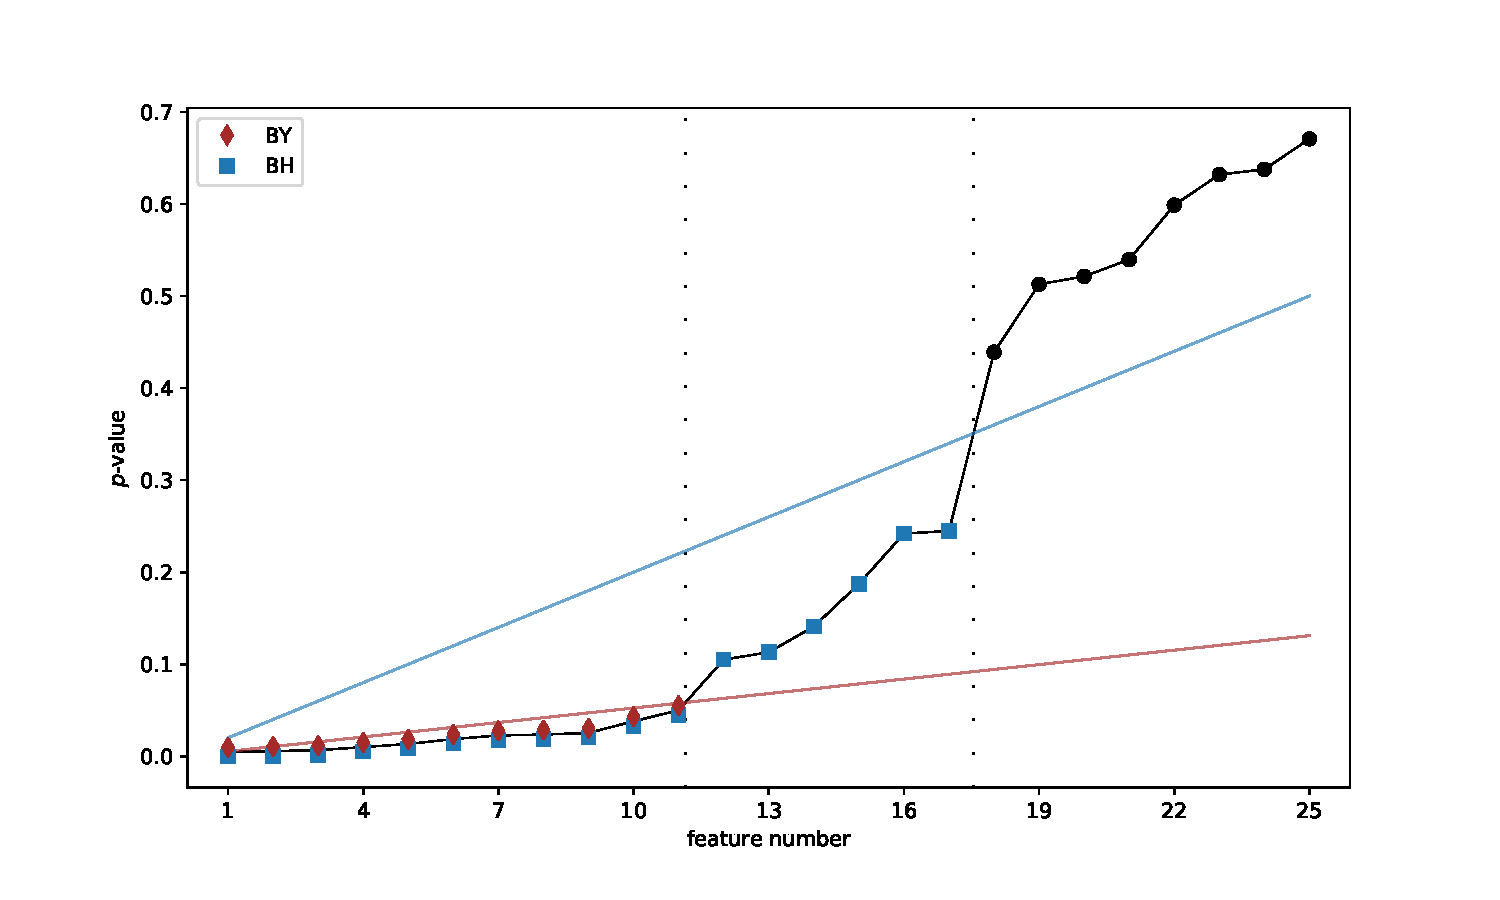
\includegraphics[width=1.\textwidth]{figures/bhy.pdf}
    \caption{
        Illustration of the BH and the BY procedures.
        Once the $p$-values are ordered,
        they are geometrically equivalent to drawing a line of slope $\beta$ going through the origin,
        identifying the last $p$-value under the line, and keeping features on its left.
        For BH, $\beta = \frac{\fdrtarget}{p}$ (in blue),
        while for BY, $\beta = \frac{\fdrtarget}{p \cdot c(p)}$ (in brown).
        In this toy example, $\fdrtarget = 0.5$, and it shows that BY is way more conservative than BH.
    }
    \label{fig:bhy}
\end{figure}
\bigbreak
Both procedures are illustrated in figure~\ref{fig:bhy}.
They require $p$-values to be computed, which is not always feasible, especially when $p > n$.
Furthermore, BH and BY have stronger guarantees than desired;
for a desired FDR level $\fdrtarget$,
they ensure that $\fdr \leq \frac{m_0}{p}\fdrtarget$,
and the factor $\frac{m_0}{p}$ might be much smaller than 1.

% \cite{statistical_inference_genome}\cite{resampled_fdr_control}\cite{unified_fdr_control}
